%%% PREAMBLE - Do not touch %%%%%%%%%%%%%%%%%%%%%%%%%%%%%%%%%%%%%%%%%%%%%%%%%%%%%%
\documentclass[10pt,twocolumn,letterpaper]{article}
\usepackage[utf8]{inputenc}
\usepackage[english]{babel}
\usepackage{model}
\usepackage{times}
\usepackage{epsfig}
\usepackage{graphicx}
\usepackage{amsmath}
\usepackage{textcomp}
\usepackage{amssymb}
\usepackage{color}
\usepackage[pagebackref=true,breaklinks=true,letterpaper=true,colorlinks,bookmarks=false]{hyperref}

%% inset source code
\usepackage{listings}

\lstset{basicstyle=\footnotesize\ttfamily,  language=Python}
\renewcommand{\lstlistingname}{Code}% Listing -> Algorithm

\let\url\nolinkurl% Make \url be equivalent to \nolinkurl
\newcommand*{\Package}[1]{\texttt{#1}}%

\cvprfinalcopy % *** Uncomment this line for the final submission
\def\httilde{\mbox{\tt\raisebox{-.5ex}{\symbol{126}}}}
\ifcvprfinal\pagestyle{empty}\fi

\newcommand{\TODO}[1]{TODO: #1}
\newcommand{\CITEONE}[2]{\mbox{#1 \cite{#2}}}
\newcommand{\CITETWO}[3]{\mbox{#1 and #2 \cite{#3}}}
\newcommand{\CITEN}[2]{\mbox{#1 et al. \cite{#2}}}

%%% Report beginning %%%%%%%%%%%%%%%%%%%%%%%%%%%%%%%%%%%%%%%%%%%%%%%%%%%%%%%%%%%%%%
\begin{document}

%%% Title and authors %%%%%%%%%%%%%%%%%%%%%%%%%%%%%%%%%%%%%%%%%%%%%%%%%%%%%%%%%%%%
\title{Relatório do projeto 1}
\author{Isadora Sophia Garcia Rodopoulos \thanks{RA 158018, Instituto de Computação, Universidade de Campinas, Unicamp. \textbf{Contact}: \tt\small{isadorasophiagr@gmail.com}} \\
Matheus Mortatti Diamantinos \thanks{RA 156740, Instituto de Computação, Universidade de Campinas, Unicamp. \textbf{Contact}: \tt\small{matdiamantino@gmail.com}}\\
Luiz Fernando Bittencourt\thanks{MC833, Instituto de Computação, Universidade de Campinas, Unicamp. \textbf{Contact}: \tt\small{bit@ic.unicamp.br }}\\
}

%%% Abstrato %%%%%%%%%%%%%%%%%%%%%%%%%%%%%%%%%%%%%%%%%%%%%%%%%%%%%%%%%%%%%%%%%%%%%
\maketitle
\begin{abstract}
O objetivo do trabalho se baseou em implementar uma estrutura de cliente e servidor que interagissem entre si.
\end{abstract}

%%% Introdução %%%%%%%%%%%%%%%%%%%%%%%%%%%%%%%%%%%%%%%%%%%%%%%%%%%%%%%%%%%%%%%%%%%
Neste projeto, foi implementado uma estrutura de comunicação entre cliente e servidor baseado em uma conexão TCP utilizando sockets na linguagem C. Nela, o cliente pode mandar mensagens de texto para o servidor que, ao confirmar o recebimento, retorna a mesma mensagem como um Acknowledge devolta ao cliente.

%%% Seções %%%%%%%#####%%%%%%%%%%%%%%%%%%%%%%%%%%%%%%%%%%%%%%%%%%%%%%%%%%%%%%%%%%%
\section{client.c}
O cliente precisa executar os seguintes passos:

 \begin{enumerate}
   \item Criar o socket de conexão
   \item Estabelecer conexão com o servidor
   \item Receber mensagem do usuário, mandar ao servidor e esperar resposta
   \item Se algum erro ocorrer ou o cliente fechar a aplicação, fechar a conexão
 \end{enumerate}

 Para isso, utilizou-se funções da library \texttt{<netdb.h>}, que nos fornece as implementações necessárias para criarmos a conexão com o servidor. A seguir, serão detalhadas as funções utilizadas e seu contexto na implementação do projeto.

\begin{enumerate}
	\item Criar o socket de conexão

	\begin{lstlisting}[caption={Função utilizada para criação do socket}, label=Algorithm]
    int socket(int domain, int type, int protocol);
	\end{lstlisting}

	\begin{lstlisting}[caption={Aplicação da função na implementação do projeto}, label=Algorithm]
    /* create active socket */
    s = socket(AF_INET, SOCK_STREAM, 0);
	\end{lstlisting}

	A função acima recebe como parâmetro a família da qual o endereço pertence (no nosso caso, IPv4), o tipo de socket (\texttt{SOCK\_STREAM}, que fornece streams de byte sequenciados, confiáveis e bidirecionais), e o protocolo a ser utilizado (0 significa que o socket vai utilizar um protocolo padrão apropriado para o tipo do socket requerido).
	

	\item Estabelecer conexão com o servidor

	Para estabelecer a conexão com o servidor, primeiramente buscamos o host baseado no endereço fornecido pelo usuário:

	\begin{lstlisting}[caption={Função utilizada para acessar o endereço do host}, label=Algorithm]
    /* get ip address */
    host_address = gethostbyname(host);
    if (host_address == NULL) {
        error("Invalid host name!\n");
    }
	\end{lstlisting}

	Esta função nos retorna o endereço do servidor na forma de \texttt{struct\_hostent}, que pode retornar \texttt{NULL} em caso de não achar o servidor.

	A variável \texttt{host address} é do tipo \texttt{hostent} especificado abaixo:

	\begin{lstlisting}[caption={Struct\_hostent}, label=Algorithm]
    struct hostent {
    	char* 	h_name;
    	char** 	h_aliases;
    	int 	h_addrtype;
    	int 	h_length;
    	char** 	h_addr_list;
    	char* 	h_addr;
    }
	\end{lstlisting}

	Contudo, apenas utilizamos \texttt{char *h\_ddr} para acessarmos o endereço do host ao realizar a conexão TCP.

	Assim, podemos utilizar a estrutura \texttt{sockaddr\_in} para especificarmos a porta e o endereço do host para a conexão:

	\begin{lstlisting}[caption={Struct sockaddr\_in}, label=Algorithm]
    
	struct sockaddr_in {
		// AF_INET, no nosso caso
	    short            sin_family;

	    // Porta de conexao
	    unsigned short   sin_port;

	    // Endereco do host
	    struct in_addr   sin_addr;
	    char             sin_zero[8];
	};

	\end{lstlisting}

	\begin{lstlisting}[caption={Implementação no Projeto}, label=Algorithm]
    
	/* initialize data address */
    bzero((char*) &socket_addr, sizeof(socket_addr));
    socket_addr.sin_family      = AF_INET;              /* ipv4 addresses */
    socket_addr.sin_port        = htons(SERVER_PORT);
    socket_addr.sin_addr = *(struct in_addr*)host_address->h_addr;

	\end{lstlisting}


	\item Receber mensagem do usuário, mandar ao servidor e esperar resposta
	\item Se algum erro ocorrer ou o cliente fechar a aplicação, fechar a conexão
 \end{enumerate}



\begin{lstlisting}[caption={Conexão do cliente com o endereço do servidor}, label=Algorithm]
python code here to show something
\end{lstlisting}

Explica mais e sei lá o que e \texttt{i can talk code too}.

\begin{lstlisting}[caption={descreva aqui}, label=Algorithm]
moar code it never ends
\end{lstlisting}

\begin{figure}[!h]
\begin{center}
    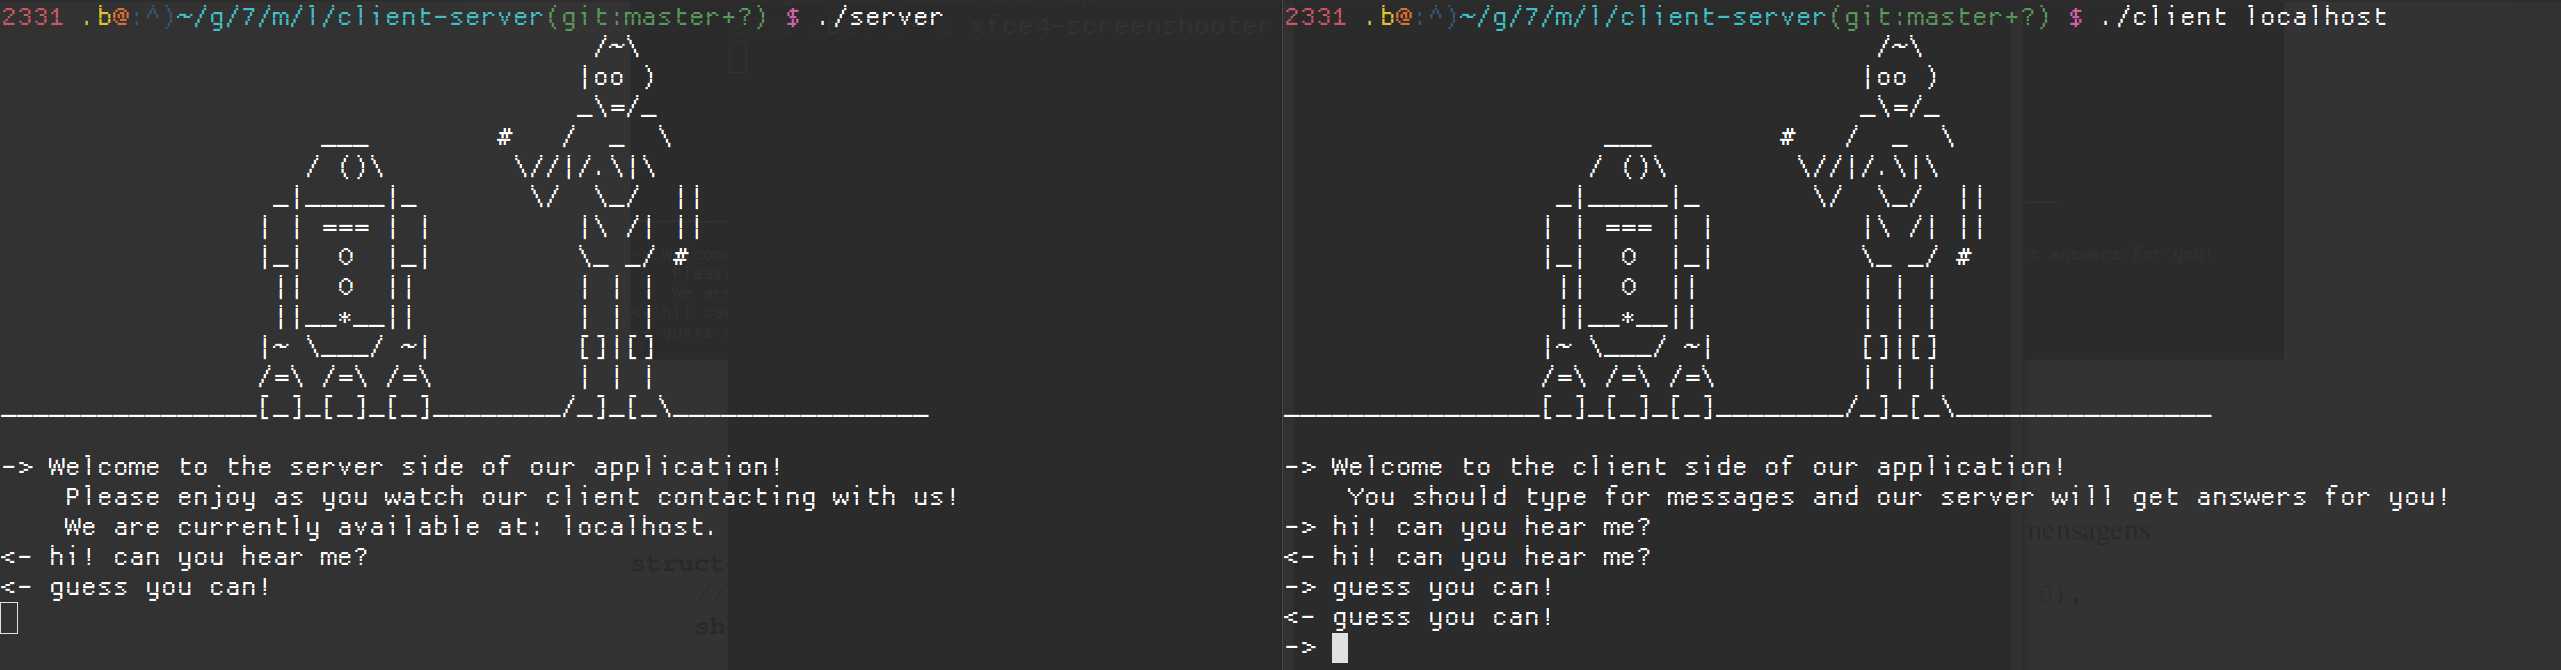
\includegraphics[width=0.45\textwidth]{img/sample.png}
    \caption{Exemplo de imagem}   
\end{center} 
\end{figure}

\section{server.c}
ablablabla aqui explica o servidor

\begin{lstlisting}[caption={aaaaaa}, label=Algorithm]
vou parar de code
\end{lstlisting}

e pretty much isso.

\section{Conclusões finais}

precisa mesmo?? coloquei mais por whatever.

%%% References %%%%%%%%%%%%%%%%%%%%%%%%%%%%%%%%%%%%%%%%%%%%%%%%%%%%%%%%%%%%%%%%%
%%
{\small
\bibliographystyle{unsrt}
\bibliography{refs}
}

\end{document}